\documentclass[twoside]{article}

% Packages required by doxygen
\usepackage{fixltx2e}
\usepackage{calc}
\usepackage{doxygen}
\usepackage{graphicx}
\usepackage[utf8]{inputenc}
\usepackage{makeidx}
\usepackage{multicol}
\usepackage{multirow}
\PassOptionsToPackage{warn}{textcomp}
\usepackage{textcomp}
\usepackage[nointegrals]{wasysym}
\usepackage[table]{xcolor}

% Font selection
\usepackage[T1]{fontenc}
\usepackage{mathptmx}
\usepackage[scaled=.90]{helvet}
\usepackage{courier}
\usepackage{amssymb}
\usepackage{sectsty}
\renewcommand{\familydefault}{\sfdefault}
\allsectionsfont{%
  \fontseries{bc}\selectfont%
  \color{darkgray}%
}
\renewcommand{\DoxyLabelFont}{%
  \fontseries{bc}\selectfont%
  \color{darkgray}%
}
\newcommand{\+}{\discretionary{\mbox{\scriptsize$\hookleftarrow$}}{}{}}

% Page & text layout
\usepackage[screen]{geometry}
\tolerance=750
\hfuzz=15pt
\hbadness=750
\setlength{\emergencystretch}{15pt}
\setlength{\parindent}{0cm}
\setlength{\parskip}{0.2cm}
\makeatletter
\renewcommand{\paragraph}{%
  \@startsection{paragraph}{4}{0ex}{-1.0ex}{1.0ex}{%
    \normalfont\normalsize\bfseries\SS@parafont%
  }%
}
\renewcommand{\subparagraph}{%
  \@startsection{subparagraph}{5}{0ex}{-1.0ex}{1.0ex}{%
    \normalfont\normalsize\bfseries\SS@subparafont%
  }%
}
\makeatother

% Headers & footers
\usepackage{fancyhdr}
\pagestyle{fancyplain}
\fancyhead[LE]{\fancyplain{}{\bfseries\thepage}}
\fancyhead[CE]{\fancyplain{}{}}
\fancyhead[RE]{\fancyplain{}{\bfseries\leftmark}}
\fancyhead[LO]{\fancyplain{}{\bfseries\rightmark}}
\fancyhead[CO]{\fancyplain{}{}}
\fancyhead[RO]{\fancyplain{}{\bfseries\thepage}}
\fancyfoot[LE]{\fancyplain{}{}}
\fancyfoot[CE]{\fancyplain{}{}}
\fancyfoot[RE]{\fancyplain{}{\bfseries\scriptsize Generated on Fri Nov 17 2017 07\+:11\+:56 by Doxygen }}
\fancyfoot[LO]{\fancyplain{}{\bfseries\scriptsize Generated on Fri Nov 17 2017 07\+:11\+:56 by Doxygen }}
\fancyfoot[CO]{\fancyplain{}{}}
\fancyfoot[RO]{\fancyplain{}{}}
\renewcommand{\footrulewidth}{0.4pt}
\renewcommand{\sectionmark}[1]{%
  \markright{\thesection\ #1}%
}

% Indices & bibliography
\usepackage{natbib}
\usepackage[titles]{tocloft}
\setcounter{tocdepth}{3}
\setcounter{secnumdepth}{5}
\makeindex

% Packages requested by user
\usepackage{titlesec}

% Hyperlinks (required, but should be loaded last)
\usepackage{ifpdf}
\ifpdf
  \usepackage[pdftex,pagebackref=true]{hyperref}
\else
  \usepackage[ps2pdf,pagebackref=true]{hyperref}
\fi
\hypersetup{%
  colorlinks=true,%
  linkcolor=blue,%
  citecolor=blue,%
  unicode%
}

% Custom commands
\newcommand{\clearemptydoublepage}{%
  \newpage{\pagestyle{empty}\cleardoublepage}%
}


\newcommand{\sectionbreak}{\clearpage}

\begin{document}

% Titlepage & ToC
\hypersetup{pageanchor=false,
             bookmarks=true,
             bookmarksnumbered=true,
             pdfencoding=unicode
            }
\pagenumbering{roman}
\begin{titlepage}
\vspace*{7cm}
\begin{center}%
{\Large Reference Manual}\\
\vspace*{1cm}
{\large Generated by Doxygen 1.8.8}\\
\vspace*{0.5cm}
{\small Fri Nov 17 2017 07:11:56}\\
\end{center}
\end{titlepage}
\tableofcontents
\pagenumbering{arabic}
\hypersetup{pageanchor=true}

%--- Begin generated contents ---
\section{Telegraph\+:\+:decode}
\label{Telegraph_1_1decode}
\hypertarget{Telegraph_1_1decode}{}
decodes morse code into english text


\begin{DoxyParams}[1]{Parameters}
\mbox{\tt in,out}  & {\em text} & A char array holding inputted or translated english text \\
\hline
\mbox{\tt in,out}  & {\em morse} & A char array holding inputted or translated morse code \\
\hline
\end{DoxyParams}
\begin{DoxyReturn}{Returns}
void 
\end{DoxyReturn}

\section{Telegraph\+:encode}
\label{Telegraph_1encode}
\hypertarget{Telegraph_1encode}{}
encodes an english message into morse code


\begin{DoxyParams}[1]{Parameters}
\mbox{\tt in,out}  & {\em text} & A char array holding inputted or translated english text \\
\hline
\mbox{\tt in,out}  & {\em morse} & A char array holding inputted or translated morse code \\
\hline
\end{DoxyParams}
\begin{DoxyReturn}{Returns}
void 
\end{DoxyReturn}

\section{Morse\+Code}
\label{MorseCode}
\hypertarget{MorseCode}{}
A struct holding letters of the alphabet along with numbers and special characters. Each symbol is associated with a morse code sequence,a max of 7 '.'s or '-\/'s total can be held in the sequence. 
\section{T\+N\+O\+D\+E}
\label{TNODE}
\hypertarget{TNODE}{}
A tree node to be used in creation of the binary tree. Used in conjunction with the open() function, when creating the tree, a tree node is made with '$\ast$' as a default symbol and no child nodes. The symbol is overwritten if the sequence ends at that tree node and child nodes are created if the sequence forces a node to be made there. 
\section{Class\+: Telegraph}
\label{Class_1_01Telegraph}
\hypertarget{Class_1_01Telegraph}{}
A class holding a table of size 40 consisting of symbols and their morse code equivalents. A root node is created automatically for creation of the binary tree. A Destroy\+Tree() function exists for the closing process of the binary tree. The class has open() and close() functions for maintaining the morse code binary tree. The class also holds encode() and decode() functions for english to morse translations and vice versa. 
\section{Telegraph\+:\+:open()}
\label{Telegraph_1_1open_07_08}
\hypertarget{Telegraph_1_1open_07_08}{}
Creates and opens a binary tree holding english symbols and their morse code equivalents

A table holding english symbols and their morse code equivalent is read. For each symbol, the morse code sequence is read and a node pointer points through the nodes depending on the sequence, creating nodes if they don't exist. If a '.' is read, it moves into the left child node of the root. If a '-\/' is read, it moves into the right child node of the root. This keeps going until the end of the sequence. For example, '.--' would cause the node pointer to point to the left child node of the root, then the right child node of the node it was pointing to, and then the left child node again of the node it was pointing to. If the nodes didn't exist, they would be created. At the end of the sequence, the symbol associated with it is stored in the node and the node pointer goes back to root, restarting the process until the table is finished. 
\section{Telegraph\+:\+:Destroy\+Tree/\+Telegraph\+:\+:close()}
\label{Telegraph_1_1DestroyTree_2Telegraph_1_1close_07_08}
\hypertarget{Telegraph_1_1DestroyTree_2Telegraph_1_1close_07_08}{}
Traverses the binary tree, deleting each node until finally deleting the root node itself

The root node is passed in and begins the deletion process. The close function calls Destroy\+Tree, a recursive function that will traverse the tree until it hits the end of both sides. Once that happens, the nodes are deleted until it reaches root. Root is then deleted, triggering the base case where a node does not exist, ending the function


\begin{DoxyParams}[1]{Parameters}
\mbox{\tt in}  & {\em $\ast$node} & The root node of the binary tree \\
\hline
\end{DoxyParams}
\begin{DoxyReturn}{Returns}
void 
\end{DoxyReturn}

\section{Specification}
\label{Specification}
\hypertarget{Specification}{}
This is the Linked List City Program. The user will see upon starting the program will see a list of cities being displayed. Then two cities will be inserted into the list and then displayed. The list will be destroyed (deleted) and then rebuilt Two new cities will then be inserted into the list and be displayed.

Freatures\+:

1) As many cities can be entered into the list as the user wants

2) The ability to add words into the dictionary/program for later use.

3) Delete/destroy list when done so one can recreate within the same program 
\section{Analysis}
\label{Analysis}
\hypertarget{Analysis}{}
When the user goes to the html page enters their information and clicks submit the program begins to run. Immediatly the translation based upon whatever the user selects will become available and the user can see it. The program is as simple as that. The code uses a binary search tree to find and create the translation. The Design section will explain this more thoroughly. 
\section{Design}
\label{Design}
\hypertarget{Design}{}
Html was what ws used to create the U\+I for this lab. we were able to have buttons to select wha we wanted and customize the page very well. Html is widely used in the industry so adopting this platfrom was the propper move. The biggest advantage I see is that I am able to edit, change, and add things very easily and I do not need the user to have certain libraries installed for them to see this. 
\section{Test\+: Morse 1}
\label{Test_1_01Morse_011}
\hypertarget{Test_1_01Morse_011}{}

\begin{DoxyImage}
\includegraphics[width=15cm]{morse1.PNG}
\caption{Morse code to be decoded}
\end{DoxyImage}
 
\section{Test\+: Morse 2}
\label{Test_1_01Morse_012}
\hypertarget{Test_1_01Morse_012}{}

\begin{DoxyImage}
\includegraphics[width=15cm]{morse2.PNG}
\caption{Morse code decoded}
\end{DoxyImage}
 
\section{Test\+: Morse Verified}
\label{Test_1_01Morse_01Verified}
\hypertarget{Test_1_01Morse_01Verified}{}

\begin{DoxyImage}
\includegraphics[width=15cm]{morse3.png}
\caption{Morse code verified}
\end{DoxyImage}
 
\section{Test\+: English 1}
\label{Test_1_01English_011}
\hypertarget{Test_1_01English_011}{}

\begin{DoxyImage}
\includegraphics[width=15cm]{english1.png}
\caption{English text to be encoded}
\end{DoxyImage}
 
\section{Test\+: English 2}
\label{Test_1_01English_012}
\hypertarget{Test_1_01English_012}{}

\begin{DoxyImage}
\includegraphics[width=15cm]{english2.png}
\caption{English text encoded}
\end{DoxyImage}
 
\section{Test\+: English Verified}
\label{Test_1_01English_01Verified}
\hypertarget{Test_1_01English_01Verified}{}

\begin{DoxyImage}
\includegraphics[width=15cm]{english3.png}
\caption{English text verified}
\end{DoxyImage}
 
\section{Morse Binary Tree}
\label{Morse_01Binary_01Tree}
\hypertarget{Morse_01Binary_01Tree}{}

\begin{DoxyImage}
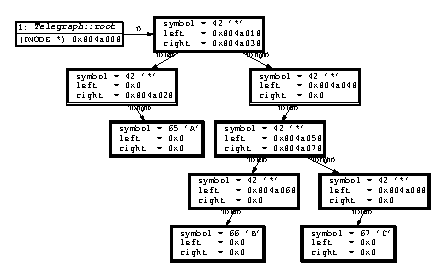
\includegraphics[width=15cm]{morseTree}
\caption{Morse Tree}
\end{DoxyImage}
 
\section{H\+T\+M\+L}
\label{HTML}
\hypertarget{HTML}{}

\begin{DoxyVerbInclude}
<!DOCTYPE html PUBLIC "-//W3C//DTD XHTML 1.0 Strict//EN" "http://www.w3.org/TR/xhtml1/DTD/xhtml1-strict.dtd">
<!-- saved from url=(0043)http://localhost:8080/cs124/lab6/morse.html -->
<html xmlns="http://www.w3.org/1999/xhtml" xml:lang="en" lang="en" wtx-context="6D7991A1-0A29-456F-A1AE-A3E37871556A"><head><meta http-equiv="Content-Type" content="text/html; charset=UTF-8">
	<title>CS 124 Lab 6 - MORSE CODE TRANSLATOR</title>
	
	<meta name="generator" content="Geany 1.24.1">
</head>

<body bgcolor="#87CEFA">
   <h1>Morse Code Translator</h1> 
   <form action="http://localhost:8080/cgi-bin/morse" wtx-context="3E5B8EA5-7244-4FCB-B3CB-CF9880D40BE8">
       <input type="text" name="e" size="50">
       <br>
       <input type="radio" name="o" value="morse">Morse Translation
       <br>
       <input type="radio" name="o" value="english">English Translation
       <br>
       <input type="submit" value="Go">
   </form>
   <!--img src="/images/graph.png"-->



</body></html>
\end{DoxyVerbInclude}
 
\section{Class Index}
\subsection{Class List}
Here are the classes, structs, unions and interfaces with brief descriptions\+:\begin{DoxyCompactList}
\item\contentsline{section}{\hyperlink{structMorseCode}{Morse\+Code} }{\pageref{structMorseCode}}{}
\item\contentsline{section}{\hyperlink{classTelegraph}{Telegraph} }{\pageref{classTelegraph}}{}
\item\contentsline{section}{\hyperlink{structTNODE}{T\+N\+O\+D\+E} }{\pageref{structTNODE}}{}
\end{DoxyCompactList}

\section{File Index}
\subsection{File List}
Here is a list of all files with brief descriptions\+:\begin{DoxyCompactList}
\item\contentsline{section}{\hyperlink{addtimes_8cpp}{addtimes.\+cpp} }{\pageref{addtimes_8cpp}}{}
\item\contentsline{section}{\hyperlink{countRows_8cpp}{count\+Rows.\+cpp} }{\pageref{countRows_8cpp}}{}
\item\contentsline{section}{\hyperlink{info_8cpp}{info.\+cpp} }{\pageref{info_8cpp}}{}
\item\contentsline{section}{\hyperlink{lab_8h}{lab.\+h} }{\pageref{lab_8h}}{}
\item\contentsline{section}{\hyperlink{main_8cpp}{main.\+cpp} }{\pageref{main_8cpp}}{}
\item\contentsline{section}{\hyperlink{overloading_8cpp}{overloading.\+cpp} }{\pageref{overloading_8cpp}}{}
\item\contentsline{section}{\hyperlink{readData_8cpp}{read\+Data.\+cpp} }{\pageref{readData_8cpp}}{}
\item\contentsline{section}{\hyperlink{readtimes_8cpp}{readtimes.\+cpp} }{\pageref{readtimes_8cpp}}{}
\item\contentsline{section}{\hyperlink{SOMETYPE_8hpp}{S\+O\+M\+E\+T\+Y\+P\+E.\+hpp} }{\pageref{SOMETYPE_8hpp}}{}
\end{DoxyCompactList}

\section{Class Documentation}
\hypertarget{structMorseCode}{\subsection{Morse\+Code Struct Reference}
\label{structMorseCode}\index{Morse\+Code@{Morse\+Code}}
}


{\ttfamily \#include $<$lab.\+h$>$}

\subsubsection*{Public Types}
\begin{DoxyCompactItemize}
\item 
enum \{ \hyperlink{structMorseCode_ab70bfb3505458b9ca361321710a3bf4ea255fc4372695bc3e775c82488bfc2dac}{N} =7
 \}
\end{DoxyCompactItemize}
\subsubsection*{Public Attributes}
\begin{DoxyCompactItemize}
\item 
char \hyperlink{structMorseCode_a15f3e521a3db80ec2f44a9c42b5cb949}{symbol}
\item 
char \hyperlink{structMorseCode_aeb273082df944b0bc60d1388f215b1b7}{code} \mbox{[}\hyperlink{structMorseCode_ab70bfb3505458b9ca361321710a3bf4ea255fc4372695bc3e775c82488bfc2dac}{N}\mbox{]}
\end{DoxyCompactItemize}


\subsubsection{Member Enumeration Documentation}
\hypertarget{structMorseCode_ab70bfb3505458b9ca361321710a3bf4e}{\paragraph[{anonymous enum}]{\setlength{\rightskip}{0pt plus 5cm}anonymous enum}}\label{structMorseCode_ab70bfb3505458b9ca361321710a3bf4e}
\begin{Desc}
\item[Enumerator]\par
\begin{description}
\index{N@{N}!Morse\+Code@{Morse\+Code}}\index{Morse\+Code@{Morse\+Code}!N@{N}}\item[{\em 
\hypertarget{structMorseCode_ab70bfb3505458b9ca361321710a3bf4ea255fc4372695bc3e775c82488bfc2dac}{N}\label{structMorseCode_ab70bfb3505458b9ca361321710a3bf4ea255fc4372695bc3e775c82488bfc2dac}
}]\end{description}
\end{Desc}

\begin{DoxyCode}
14 \{\hyperlink{structMorseCode_ab70bfb3505458b9ca361321710a3bf4ea255fc4372695bc3e775c82488bfc2dac}{N}=7\};
\end{DoxyCode}


\subsubsection{Member Data Documentation}
\hypertarget{structMorseCode_aeb273082df944b0bc60d1388f215b1b7}{\index{Morse\+Code@{Morse\+Code}!code@{code}}
\index{code@{code}!Morse\+Code@{Morse\+Code}}
\paragraph[{code}]{\setlength{\rightskip}{0pt plus 5cm}char Morse\+Code\+::code\mbox{[}{\bf N}\mbox{]}}}\label{structMorseCode_aeb273082df944b0bc60d1388f215b1b7}
\hypertarget{structMorseCode_a15f3e521a3db80ec2f44a9c42b5cb949}{\index{Morse\+Code@{Morse\+Code}!symbol@{symbol}}
\index{symbol@{symbol}!Morse\+Code@{Morse\+Code}}
\paragraph[{symbol}]{\setlength{\rightskip}{0pt plus 5cm}char Morse\+Code\+::symbol}}\label{structMorseCode_a15f3e521a3db80ec2f44a9c42b5cb949}


The documentation for this struct was generated from the following file\+:\begin{DoxyCompactItemize}
\item 
\hyperlink{lab_8h}{lab.\+h}\end{DoxyCompactItemize}

\hypertarget{classTelegraph}{\subsection{Telegraph Class Reference}
\label{classTelegraph}\index{Telegraph@{Telegraph}}
}


{\ttfamily \#include $<$lab.\+h$>$}

\subsubsection*{Public Member Functions}
\begin{DoxyCompactItemize}
\item 
void \hyperlink{classTelegraph_ac076aaff18187105bbc553302cf630d5}{encode} (char text\mbox{[}$\,$\mbox{]}, char morse\mbox{[}$\,$\mbox{]})
\item 
void \hyperlink{classTelegraph_a131e9c2acc739501496b9b7f48e833aa}{decode} (char morse\mbox{[}$\,$\mbox{]}, char text\mbox{[}$\,$\mbox{]})
\end{DoxyCompactItemize}
\subsubsection*{Static Public Member Functions}
\begin{DoxyCompactItemize}
\item 
static void \hyperlink{classTelegraph_a2ace7d6ba4d3742dbcc57d6a36a13b54}{open} ()
\item 
static void \hyperlink{classTelegraph_a5a49093b588a538d53449aba1e66f44c}{close} ()
\end{DoxyCompactItemize}


\subsubsection{Member Function Documentation}
\hypertarget{classTelegraph_a5a49093b588a538d53449aba1e66f44c}{\index{Telegraph@{Telegraph}!close@{close}}
\index{close@{close}!Telegraph@{Telegraph}}
\paragraph[{close}]{\setlength{\rightskip}{0pt plus 5cm}static void Telegraph\+::close (
\begin{DoxyParamCaption}
{}
\end{DoxyParamCaption}
)\hspace{0.3cm}{\ttfamily [inline]}, {\ttfamily [static]}}}\label{classTelegraph_a5a49093b588a538d53449aba1e66f44c}

\begin{DoxyCode}
56 \{ DestroyTree(root); \}
\end{DoxyCode}
\hypertarget{classTelegraph_a131e9c2acc739501496b9b7f48e833aa}{\index{Telegraph@{Telegraph}!decode@{decode}}
\index{decode@{decode}!Telegraph@{Telegraph}}
\paragraph[{decode}]{\setlength{\rightskip}{0pt plus 5cm}void Telegraph\+::decode (
\begin{DoxyParamCaption}
\item[{char}]{morse\mbox{[}$\,$\mbox{]}, }
\item[{char}]{text\mbox{[}$\,$\mbox{]}}
\end{DoxyParamCaption}
)}}\label{classTelegraph_a131e9c2acc739501496b9b7f48e833aa}

\begin{DoxyCode}
10 \{
11     \textcolor{keywordtype}{char} *dd;
12     \textcolor{keywordtype}{int} count = 0;
13     \hyperlink{structTNODE}{TNODE} *node;
14     
15     node = root;
16     \textcolor{keywordflow}{for}(dd = morse; *dd; dd++) \{
17         \textcolor{keywordflow}{if}(*dd == \textcolor{charliteral}{'.'}) 
18             node = node->\hyperlink{structTNODE_ac8548d0ee2d54b914e0e07ab35375dba}{left};
19         \textcolor{keywordflow}{else} \textcolor{keywordflow}{if}(*dd == \textcolor{charliteral}{'-'})
20             node = node->\hyperlink{structTNODE_a4e135d9137519b2a4b89dbccb55ae967}{right};
21         \textcolor{keywordflow}{else} \textcolor{keywordflow}{if}(*dd == \textcolor{charliteral}{'/'}) \{
22             node->\hyperlink{structTNODE_a436db20d992c4227b8482603b4f76712}{symbol} = \textcolor{charliteral}{' '};
23         \}   
24         \textcolor{keywordflow}{else} \{
25             text[count] = node->\hyperlink{structTNODE_a436db20d992c4227b8482603b4f76712}{symbol};
26             node = root;
27             count++;
28         \}
29     \}
30 \}
\end{DoxyCode}
\hypertarget{classTelegraph_ac076aaff18187105bbc553302cf630d5}{\index{Telegraph@{Telegraph}!encode@{encode}}
\index{encode@{encode}!Telegraph@{Telegraph}}
\paragraph[{encode}]{\setlength{\rightskip}{0pt plus 5cm}void Telegraph\+::encode (
\begin{DoxyParamCaption}
\item[{char}]{text\mbox{[}$\,$\mbox{]}, }
\item[{char}]{morse\mbox{[}$\,$\mbox{]}}
\end{DoxyParamCaption}
)}}\label{classTelegraph_ac076aaff18187105bbc553302cf630d5}

\begin{DoxyCode}
10 \{
11     \textcolor{keywordtype}{int} i;
12     \textcolor{keywordtype}{char} c, *t, *dd; \textcolor{comment}{// t points to text}
13                      \textcolor{comment}{// dd points to a string of dots and dashes}
14     \textcolor{keywordflow}{for}(t = text; *t; t++)
15     \{
16         
17         c = toupper(*t);
18         
19         \textcolor{comment}{// If space, add a space to the morse string:}
20         \textcolor{keywordflow}{if}(c == \textcolor{charliteral}{' '}) \{
21             *morse++ = \textcolor{charliteral}{'/'};
22             *morse++ = \textcolor{charliteral}{' '};
23             \textcolor{keywordflow}{continue};
24         \}
25         
26         \textcolor{comment}{// Find this symbol in the MORSECODE table}
27         \textcolor{comment}{// skip this symbol if not found:}
28         \textcolor{keywordflow}{for}(i = 0; table[i].\hyperlink{structMorseCode_a15f3e521a3db80ec2f44a9c42b5cb949}{symbol}; i++)
29             \textcolor{keywordflow}{if}(table[i].symbol == c) \textcolor{keywordflow}{break};
30         \textcolor{keywordflow}{if}(!table[i].symbol) \textcolor{keywordflow}{continue};
31         
32         \textcolor{comment}{// Copy its code into the morse string:}
33         dd = table[i].\hyperlink{structMorseCode_aeb273082df944b0bc60d1388f215b1b7}{code};
34        
35         \textcolor{keywordflow}{while}(*dd) *morse++=*dd++;
36         
37         \textcolor{comment}{// Add one space to separate letters:}
38         *morse++ = \textcolor{charliteral}{' '};
39     \}
40     *morse = \textcolor{charliteral}{'\(\backslash\)0'};
41 \}
\end{DoxyCode}
\hypertarget{classTelegraph_a2ace7d6ba4d3742dbcc57d6a36a13b54}{\index{Telegraph@{Telegraph}!open@{open}}
\index{open@{open}!Telegraph@{Telegraph}}
\paragraph[{open}]{\setlength{\rightskip}{0pt plus 5cm}void Telegraph\+::open (
\begin{DoxyParamCaption}
{}
\end{DoxyParamCaption}
)\hspace{0.3cm}{\ttfamily [static]}}}\label{classTelegraph_a2ace7d6ba4d3742dbcc57d6a36a13b54}

\begin{DoxyCode}
39 \{
40     \textcolor{keywordtype}{char}* dd;
41     Telegraph::root = \textcolor{keyword}{new} \hyperlink{structTNODE}{TNODE};
42     \hyperlink{structTNODE}{TNODE}* node; \hyperlink{structTNODE}{TNODE}* nextnode;
43     \textcolor{keywordflow}{for}(\textcolor{keywordtype}{int} i = 0; i < N; i++) \{
44         node = root;
45         \textcolor{keywordflow}{for}( dd = table[i].code; *dd; dd++) \{
46                 
47             \textcolor{keywordflow}{if}(*dd == \textcolor{charliteral}{'.'}) 
48             \{
49                 nextnode = node->\hyperlink{structTNODE_ac8548d0ee2d54b914e0e07ab35375dba}{left};
50                 \textcolor{keywordflow}{if}(not nextnode) 
51                 \{
52                 nextnode = \textcolor{keyword}{new} \hyperlink{structTNODE}{TNODE};
53                 node-> left = nextnode;
54                 \}
55             \}
56             \textcolor{keywordflow}{else} \textcolor{keywordflow}{if}(*dd == \textcolor{charliteral}{'-'})
57              \{
58                 nextnode = node->\hyperlink{structTNODE_a4e135d9137519b2a4b89dbccb55ae967}{right};
59                 \textcolor{keywordflow}{if}(not nextnode) 
60                 \{
61                 nextnode = \textcolor{keyword}{new} \hyperlink{structTNODE}{TNODE};
62                 node-> right = nextnode;
63                 \}
64             \}
65             \textcolor{keywordflow}{else} std::cerr << \textcolor{stringliteral}{"Unknown morse code"} << std::endl;
66             node = nextnode;
67          \} \textcolor{comment}{//not dash or dot, must be null so assign symbol}
68          node->\hyperlink{structTNODE_a436db20d992c4227b8482603b4f76712}{symbol} = table[i].\hyperlink{structMorseCode_a15f3e521a3db80ec2f44a9c42b5cb949}{symbol};
69     \}
70 \}
\end{DoxyCode}


The documentation for this class was generated from the following files\+:\begin{DoxyCompactItemize}
\item 
\hyperlink{lab_8h}{lab.\+h}\item 
\hyperlink{decode_8cpp}{decode.\+cpp}\item 
\hyperlink{encode_8cpp}{encode.\+cpp}\item 
\hyperlink{morse_8cpp}{morse.\+cpp}\end{DoxyCompactItemize}

\hypertarget{structTNODE}{\subsection{T\+N\+O\+D\+E Struct Reference}
\label{structTNODE}\index{T\+N\+O\+D\+E@{T\+N\+O\+D\+E}}
}


{\ttfamily \#include $<$lab.\+h$>$}



Collaboration diagram for T\+N\+O\+D\+E\+:\nopagebreak
\begin{figure}[H]
\begin{center}
\leavevmode
\includegraphics[width=172pt]{structTNODE__coll__graph}
\end{center}
\end{figure}
\subsubsection*{Public Member Functions}
\begin{DoxyCompactItemize}
\item 
\hyperlink{structTNODE_a0f2d73dc28ef3be182dbb07464560a47}{T\+N\+O\+D\+E} ()
\end{DoxyCompactItemize}
\subsubsection*{Public Attributes}
\begin{DoxyCompactItemize}
\item 
char \hyperlink{structTNODE_a436db20d992c4227b8482603b4f76712}{symbol}
\item 
\hyperlink{structTNODE}{T\+N\+O\+D\+E} $\ast$ \hyperlink{structTNODE_ac8548d0ee2d54b914e0e07ab35375dba}{left}
\item 
\hyperlink{structTNODE}{T\+N\+O\+D\+E} $\ast$ \hyperlink{structTNODE_a4e135d9137519b2a4b89dbccb55ae967}{right}
\end{DoxyCompactItemize}


\subsubsection{Constructor \& Destructor Documentation}
\hypertarget{structTNODE_a0f2d73dc28ef3be182dbb07464560a47}{\index{T\+N\+O\+D\+E@{T\+N\+O\+D\+E}!T\+N\+O\+D\+E@{T\+N\+O\+D\+E}}
\index{T\+N\+O\+D\+E@{T\+N\+O\+D\+E}!T\+N\+O\+D\+E@{T\+N\+O\+D\+E}}
\paragraph[{T\+N\+O\+D\+E}]{\setlength{\rightskip}{0pt plus 5cm}T\+N\+O\+D\+E\+::\+T\+N\+O\+D\+E (
\begin{DoxyParamCaption}
{}
\end{DoxyParamCaption}
)\hspace{0.3cm}{\ttfamily [inline]}}}\label{structTNODE_a0f2d73dc28ef3be182dbb07464560a47}

\begin{DoxyCode}
31              \{
32         \hyperlink{structTNODE_a436db20d992c4227b8482603b4f76712}{symbol} = \textcolor{charliteral}{'*'};
33         \hyperlink{structTNODE_ac8548d0ee2d54b914e0e07ab35375dba}{left} = 0;
34         \hyperlink{structTNODE_a4e135d9137519b2a4b89dbccb55ae967}{right} = 0;
35     \}
\end{DoxyCode}


\subsubsection{Member Data Documentation}
\hypertarget{structTNODE_ac8548d0ee2d54b914e0e07ab35375dba}{\index{T\+N\+O\+D\+E@{T\+N\+O\+D\+E}!left@{left}}
\index{left@{left}!T\+N\+O\+D\+E@{T\+N\+O\+D\+E}}
\paragraph[{left}]{\setlength{\rightskip}{0pt plus 5cm}{\bf T\+N\+O\+D\+E}$\ast$ T\+N\+O\+D\+E\+::left}}\label{structTNODE_ac8548d0ee2d54b914e0e07ab35375dba}
\hypertarget{structTNODE_a4e135d9137519b2a4b89dbccb55ae967}{\index{T\+N\+O\+D\+E@{T\+N\+O\+D\+E}!right@{right}}
\index{right@{right}!T\+N\+O\+D\+E@{T\+N\+O\+D\+E}}
\paragraph[{right}]{\setlength{\rightskip}{0pt plus 5cm}{\bf T\+N\+O\+D\+E}$\ast$ T\+N\+O\+D\+E\+::right}}\label{structTNODE_a4e135d9137519b2a4b89dbccb55ae967}
\hypertarget{structTNODE_a436db20d992c4227b8482603b4f76712}{\index{T\+N\+O\+D\+E@{T\+N\+O\+D\+E}!symbol@{symbol}}
\index{symbol@{symbol}!T\+N\+O\+D\+E@{T\+N\+O\+D\+E}}
\paragraph[{symbol}]{\setlength{\rightskip}{0pt plus 5cm}char T\+N\+O\+D\+E\+::symbol}}\label{structTNODE_a436db20d992c4227b8482603b4f76712}


The documentation for this struct was generated from the following file\+:\begin{DoxyCompactItemize}
\item 
\hyperlink{lab_8h}{lab.\+h}\end{DoxyCompactItemize}

\section{File Documentation}
\hypertarget{decode_8cpp}{\subsection{decode.\+cpp File Reference}
\label{decode_8cpp}\index{decode.\+cpp@{decode.\+cpp}}
}
{\ttfamily \#include \char`\"{}lab.\+h\char`\"{}}\\*

\hypertarget{encode_8cpp}{\subsection{encode.\+cpp File Reference}
\label{encode_8cpp}\index{encode.\+cpp@{encode.\+cpp}}
}
{\ttfamily \#include \char`\"{}lab.\+h\char`\"{}}\\*

\hypertarget{lab_8h}{\subsection{lab.\+h File Reference}
\label{lab_8h}\index{lab.\+h@{lab.\+h}}
}
{\ttfamily \#include $<$iostream$>$}\\*
{\ttfamily \#include $<$string$>$}\\*
{\ttfamily \#include \char`\"{}config.\+h\char`\"{}}\\*
{\ttfamily \#include $<$F\+L/\+Fl\+\_\+\+Cairo\+\_\+\+Window.\+H$>$}\\*
{\ttfamily \#include $<$F\+L/\+Fl\+\_\+\+Input.\+H$>$}\\*
{\ttfamily \#include $<$F\+L/\+Fl\+\_\+\+Button.\+H$>$}\\*
{\ttfamily \#include $<$F\+L/fl\+\_\+ask.\+H$>$}\\*
{\ttfamily \#include $<$F\+L/\+Fl\+\_\+\+Output.\+H$>$}\\*
{\ttfamily \#include $<$sstream$>$}\\*
{\ttfamily \#include $<$iomanip$>$}\\*
{\ttfamily \#include $<$Fl/\+Fl\+\_\+\+Text\+\_\+\+Display.\+H$>$}\\*
{\ttfamily \#include $<$Fl/\+Fl\+\_\+\+Text\+\_\+\+Buffer.\+H$>$}\\*
Include dependency graph for lab.\+h\+:\nopagebreak
\begin{figure}[H]
\begin{center}
\leavevmode
\includegraphics[width=350pt]{lab_8h__incl}
\end{center}
\end{figure}
This graph shows which files directly or indirectly include this file\+:\nopagebreak
\begin{figure}[H]
\begin{center}
\leavevmode
\includegraphics[width=350pt]{lab_8h__dep__incl}
\end{center}
\end{figure}
\subsubsection*{Classes}
\begin{DoxyCompactItemize}
\item 
struct \hyperlink{structORDER}{O\+R\+D\+E\+R}
\item 
struct \hyperlink{structNODE}{N\+O\+D\+E}
\item 
class \hyperlink{classLLQUEUE}{L\+L\+Q\+U\+E\+U\+E}
\item 
class \hyperlink{classRBQUEUE}{R\+B\+Q\+U\+E\+U\+E}
\end{DoxyCompactItemize}
\subsubsection*{Functions}
\begin{DoxyCompactItemize}
\item 
void \hyperlink{lab_8h_a14029123842f0c00bf955eaeea529b17}{order\+Cb} (Fl\+\_\+\+Callback, void $\ast$)
\item 
void \hyperlink{lab_8h_aa05ac27c7de405a78817cddb14e9f303}{driver\+Cb} (Fl\+\_\+\+Callback, void $\ast$)
\item 
void \hyperlink{lab_8h_a56ac87e7157d59fc25975adae5b10cb6}{show\+Q} (Fl\+\_\+\+Callback $\ast$, void $\ast$)
\item 
void \hyperlink{lab_8h_a2d579cefafebe0f193a6a3ea99f4d1c6}{deliver} (void $\ast$)
\item 
Fl\+\_\+\+Cairo\+\_\+\+Window $\ast$ \hyperlink{lab_8h_af7bd238954bf4d2d0f780d4d80eaf2b2}{window} ()
\end{DoxyCompactItemize}
\subsubsection*{Variables}
\begin{DoxyCompactItemize}
\item 
const int \hyperlink{lab_8h_a66326676d44c838441a4dc39c85f599b}{w} = 300
\item 
const int \hyperlink{lab_8h_a3f40fea9b1040e381f08ddd4b026765d}{h} = 300
\item 
const int \hyperlink{lab_8h_ad69f678058ac1e2c6d82212fd735b7a4}{B\+U\+F\+S\+I\+Z\+E} = 10
\item 
Fl\+\_\+\+Input $\ast$ \hyperlink{lab_8h_abf805c82a90897837d1c26ef915f1cd6}{pizza}
\item 
Fl\+\_\+\+Input $\ast$ \hyperlink{lab_8h_a0ce7586472726848924b4964b80e69ba}{address}
\item 
Fl\+\_\+\+Input $\ast$ \hyperlink{lab_8h_ac3a31ef741b6d40c85fd634017661a38}{Driver}
\item 
Fl\+\_\+\+Output $\ast$ \hyperlink{lab_8h_a05c7f6e86cca5f4d0ebf44d1f5042c37}{watch}
\item 
Fl\+\_\+\+Text\+\_\+\+Buffer $\ast$ \hyperlink{lab_8h_aea2b8efadc87a819fe57c311d668e504}{buff}
\item 
Fl\+\_\+\+Text\+\_\+\+Display $\ast$ \hyperlink{lab_8h_a23f917547a833922fd6bc8797cc04ee1}{order\+Q}
\item 
\hyperlink{structORDER}{O\+R\+D\+E\+R} \hyperlink{lab_8h_a9b6b9e3013897906bcd799b34de83de3}{order}
\item 
\hyperlink{classLLQUEUE}{L\+L\+Q\+U\+E\+U\+E} \hyperlink{lab_8h_af9cad0e28281b8add71f55142323def6}{pending\+Order}
\item 
\hyperlink{classRBQUEUE}{R\+B\+Q\+U\+E\+U\+E} \hyperlink{lab_8h_a3dc8498494666cf6c70359b55fe9202c}{drivers}
\end{DoxyCompactItemize}


\subsubsection{Function Documentation}
\hypertarget{lab_8h_a2d579cefafebe0f193a6a3ea99f4d1c6}{\index{lab.\+h@{lab.\+h}!deliver@{deliver}}
\index{deliver@{deliver}!lab.\+h@{lab.\+h}}
\paragraph[{deliver}]{\setlength{\rightskip}{0pt plus 5cm}void deliver (
\begin{DoxyParamCaption}
\item[{void $\ast$}]{}
\end{DoxyParamCaption}
)}}\label{lab_8h_a2d579cefafebe0f193a6a3ea99f4d1c6}
This function will put out alerts when drivers or Orders are ready See the comments for more details. The message displayed is based on which of the queues are empty. This wee then cause the message to be displayed. 
\begin{DoxyCode}
10 \{
11     
12     \textcolor{keywordtype}{string} driverName;
13     
14     
15     \textcolor{keywordflow}{if}(!\hyperlink{lab_8h_af9cad0e28281b8add71f55142323def6}{pendingOrder}.\hyperlink{classLLQUEUE_acf5810657663dfbb5ac62407bd78950c}{isEmpty}() && !\hyperlink{lab_8h_a3dc8498494666cf6c70359b55fe9202c}{drivers}.\hyperlink{classRBQUEUE_a3a97717d7831d8489981beceafac4122}{isEmpty}())
16     \{
17         \hyperlink{lab_8h_a3dc8498494666cf6c70359b55fe9202c}{drivers}.\hyperlink{classRBQUEUE_a53ab97610e4b96c9548d2ffe38108631}{Remove}(driverName);
18         \hyperlink{lab_8h_af9cad0e28281b8add71f55142323def6}{pendingOrder}.\hyperlink{classLLQUEUE_ab8d52943d24188adf0855a0ee9fa0afe}{Remove}(\hyperlink{lab_8h_a9b6b9e3013897906bcd799b34de83de3}{order});
19         
20         \textcolor{keywordtype}{string} alert = driverName + \textcolor{stringliteral}{", deliver one "} + \hyperlink{lab_8h_a9b6b9e3013897906bcd799b34de83de3}{order}.\hyperlink{structORDER_a244508e0d34d5da2b9ff18a5e02cbcf9}{items}
21         + \textcolor{stringliteral}{" pizza at "} + \hyperlink{lab_8h_a9b6b9e3013897906bcd799b34de83de3}{order}.\hyperlink{structORDER_a6b9ce0a29de13c2c2f1721627dba4812}{address}; \textcolor{comment}{// create the string for the alert}
22         
23         cout << alert << endl;
24         
25         fl\_message\_title(\textcolor{stringliteral}{"Pizza Time!"});
26         fl\_message(alert.c\_str()); \textcolor{comment}{//add in the message}
27         Fl::repeat\_timeout(5.0,\hyperlink{deliver_8cpp_a2d579cefafebe0f193a6a3ea99f4d1c6}{deliver}); \textcolor{comment}{//display it}
28         
29     \}
30     
31     \textcolor{keywordflow}{else} \textcolor{keywordflow}{if} (!\hyperlink{lab_8h_af9cad0e28281b8add71f55142323def6}{pendingOrder}.\hyperlink{classLLQUEUE_acf5810657663dfbb5ac62407bd78950c}{isEmpty}() && \hyperlink{lab_8h_a3dc8498494666cf6c70359b55fe9202c}{drivers}.
      \hyperlink{classRBQUEUE_a3a97717d7831d8489981beceafac4122}{isEmpty}())
32     \{
33         
34         \textcolor{keywordtype}{string} alert1 =\textcolor{stringliteral}{"Delivery for one "} + \hyperlink{lab_8h_a9b6b9e3013897906bcd799b34de83de3}{order}.\hyperlink{structORDER_a244508e0d34d5da2b9ff18a5e02cbcf9}{items}
35         + \textcolor{stringliteral}{" pizza at "} + \hyperlink{lab_8h_a9b6b9e3013897906bcd799b34de83de3}{order}.\hyperlink{structORDER_a6b9ce0a29de13c2c2f1721627dba4812}{address}; \textcolor{comment}{//Create the string for the message}
36         
37         cout << alert1 << endl;
38         
39         fl\_message\_title(\textcolor{stringliteral}{"Pizza Time!"});
40         fl\_message(alert1.c\_str()); \textcolor{comment}{// Add the message into the alert}
41         Fl::repeat\_timeout(5.0,\hyperlink{deliver_8cpp_a2d579cefafebe0f193a6a3ea99f4d1c6}{deliver}); \textcolor{comment}{//display it}
42         
43         
44         
45     \}
46     
47      \textcolor{keywordflow}{else} \textcolor{keywordflow}{if} (\hyperlink{lab_8h_af9cad0e28281b8add71f55142323def6}{pendingOrder}.\hyperlink{classLLQUEUE_acf5810657663dfbb5ac62407bd78950c}{isEmpty}() && !\hyperlink{lab_8h_a3dc8498494666cf6c70359b55fe9202c}{drivers}.
      \hyperlink{classRBQUEUE_a3a97717d7831d8489981beceafac4122}{isEmpty}())
48     \{
49         
50         \textcolor{keywordtype}{string} alert2 = driverName + \textcolor{stringliteral}{" is now available"};
51         
52         cout << alert2 << endl;
53         
54         fl\_message\_title(\textcolor{stringliteral}{"Pizza Time!"});
55         fl\_message(alert2.c\_str());
56         Fl::repeat\_timeout(5.0,\hyperlink{deliver_8cpp_a2d579cefafebe0f193a6a3ea99f4d1c6}{deliver});
57         
58         
59         
60     \}
61 
62 
63 \}
\end{DoxyCode}
\hypertarget{lab_8h_aa05ac27c7de405a78817cddb14e9f303}{\index{lab.\+h@{lab.\+h}!driver\+Cb@{driver\+Cb}}
\index{driver\+Cb@{driver\+Cb}!lab.\+h@{lab.\+h}}
\paragraph[{driver\+Cb}]{\setlength{\rightskip}{0pt plus 5cm}void driver\+Cb (
\begin{DoxyParamCaption}
\item[{Fl\+\_\+\+Callback}]{, }
\item[{void $\ast$}]{}
\end{DoxyParamCaption}
)}}\label{lab_8h_aa05ac27c7de405a78817cddb14e9f303}
\hypertarget{lab_8h_a14029123842f0c00bf955eaeea529b17}{\index{lab.\+h@{lab.\+h}!order\+Cb@{order\+Cb}}
\index{order\+Cb@{order\+Cb}!lab.\+h@{lab.\+h}}
\paragraph[{order\+Cb}]{\setlength{\rightskip}{0pt plus 5cm}void order\+Cb (
\begin{DoxyParamCaption}
\item[{Fl\+\_\+\+Callback}]{, }
\item[{void $\ast$}]{}
\end{DoxyParamCaption}
)}}\label{lab_8h_a14029123842f0c00bf955eaeea529b17}
\hypertarget{lab_8h_a56ac87e7157d59fc25975adae5b10cb6}{\index{lab.\+h@{lab.\+h}!show\+Q@{show\+Q}}
\index{show\+Q@{show\+Q}!lab.\+h@{lab.\+h}}
\paragraph[{show\+Q}]{\setlength{\rightskip}{0pt plus 5cm}void show\+Q (
\begin{DoxyParamCaption}
\item[{Fl\+\_\+\+Callback $\ast$}]{, }
\item[{void $\ast$}]{}
\end{DoxyParamCaption}
)}}\label{lab_8h_a56ac87e7157d59fc25975adae5b10cb6}
This function shows the the queues when the user presses Track order in the G\+U\+I. This function shows the addresses and the pizza as well as the drivers that are available. 
\begin{DoxyCode}
8 \{
9     \textcolor{keywordtype}{string} orderlist;
10     \textcolor{keywordtype}{string} driverlist;
11     
12     \textcolor{keyword}{static} Fl\_Cairo\_Window trackWindow(200, 200); \textcolor{comment}{//Build the window}
13     trackWindow.label(\textcolor{stringliteral}{"Tracking Orders"});
14     \textcolor{keyword}{static} Fl\_Text\_Buffer \hyperlink{lab_8h_aea2b8efadc87a819fe57c311d668e504}{buff};
15     \textcolor{keyword}{static} Fl\_Text\_Display OrderQ(0,0, 200,200, \textcolor{stringliteral}{"Track Order:"});
16     OrderQ.buffer(&buff);
17     
18     \textcolor{keywordtype}{string} o = \hyperlink{lab_8h_af9cad0e28281b8add71f55142323def6}{pendingOrder}.\hyperlink{classLLQUEUE_ac2b49f6579d59d4de02c17f456aa6f5e}{traverse}(\hyperlink{lab_8h_a9b6b9e3013897906bcd799b34de83de3}{order}); \textcolor{comment}{//using the traverse fucntion to
       creat the list}
19     \textcolor{keywordtype}{string} d = \hyperlink{lab_8h_a3dc8498494666cf6c70359b55fe9202c}{drivers}.\hyperlink{classRBQUEUE_ae554aac84a4435a51a5d0029050c30e3}{traverse}();
20     o+=d;\textcolor{comment}{//This creates the list of Orders and Drivers}
21     
22     buff.text(o.c\_str());
23     trackWindow.add(OrderQ);
24     trackWindow.show(); \textcolor{comment}{//Displays the window}
25 \}
\end{DoxyCode}
\hypertarget{lab_8h_af7bd238954bf4d2d0f780d4d80eaf2b2}{\index{lab.\+h@{lab.\+h}!window@{window}}
\index{window@{window}!lab.\+h@{lab.\+h}}
\paragraph[{window}]{\setlength{\rightskip}{0pt plus 5cm}Fl\+\_\+\+Cairo\+\_\+\+Window$\ast$ window (
\begin{DoxyParamCaption}
{}
\end{DoxyParamCaption}
)}}\label{lab_8h_af7bd238954bf4d2d0f780d4d80eaf2b2}

\begin{DoxyCode}
18 \{
19     \hyperlink{window_8cpp_a5fe2ac8fad8e5bd201410fafd75eae23}{cw} = \textcolor{keyword}{new} Fl\_Cairo\_Window(\hyperlink{lab_8h_a66326676d44c838441a4dc39c85f599b}{w},\hyperlink{lab_8h_a3f40fea9b1040e381f08ddd4b026765d}{h});
20     
21     \hyperlink{window_8cpp_a5fe2ac8fad8e5bd201410fafd75eae23}{cw}->label(\textcolor{stringliteral}{"Pizza Delivery Services"});
22     
23     \hyperlink{window_8cpp_a5fe2ac8fad8e5bd201410fafd75eae23}{cw}->color(FL\_GRAY);
24     
25     \hyperlink{window_8cpp_af7bb2b2233230b6a112892f626be3a2d}{Order} = \textcolor{keyword}{new} Fl\_Button(200,40,70,20,\textcolor{stringliteral}{"Order"});
26     \hyperlink{window_8cpp_af7bb2b2233230b6a112892f626be3a2d}{Order}->callback((Fl\_Callback*)\hyperlink{lab_8h_a14029123842f0c00bf955eaeea529b17}{orderCb});
27     
28     \hyperlink{window_8cpp_a6737b513e36303ae81b9f65206239dec}{driver} = \textcolor{keyword}{new} Fl\_Button(200,90,70,20,\textcolor{stringliteral}{"Driver"});
29     \hyperlink{window_8cpp_a6737b513e36303ae81b9f65206239dec}{driver}->callback((Fl\_Callback*)\hyperlink{driverCb_8cpp_a9c6487e79c76ee9ad1efcb3e0e91ad93}{driverCb});
30     
31     \hyperlink{window_8cpp_a9cae10bde8006c09e5a662d92cb81999}{tracker} = \textcolor{keyword}{new} Fl\_Button (150,130,90,30,\textcolor{stringliteral}{"Track Order"});
32     \hyperlink{window_8cpp_a9cae10bde8006c09e5a662d92cb81999}{tracker}->callback((Fl\_Callback*)\hyperlink{lab_8h_a56ac87e7157d59fc25975adae5b10cb6}{showQ});
33     
34     \hyperlink{window_8cpp_abf805c82a90897837d1c26ef915f1cd6}{pizza} = \textcolor{keyword}{new} Fl\_Input(80,20,100,20,\textcolor{stringliteral}{"Pizza: "});
35     \hyperlink{window_8cpp_abf805c82a90897837d1c26ef915f1cd6}{pizza} -> color(FL\_WHITE);
36     
37     \hyperlink{window_8cpp_a0ce7586472726848924b4964b80e69ba}{address} = \textcolor{keyword}{new} Fl\_Input(80,40,100,20, \textcolor{stringliteral}{"Address: "});
38     \hyperlink{window_8cpp_a0ce7586472726848924b4964b80e69ba}{address}-> color(FL\_WHITE);
39     
40     \hyperlink{window_8cpp_ac3a31ef741b6d40c85fd634017661a38}{Driver} = \textcolor{keyword}{new} Fl\_Input(80,80,100,20, \textcolor{stringliteral}{"Driver: "});
41     \hyperlink{window_8cpp_ac3a31ef741b6d40c85fd634017661a38}{Driver}-> color(FL\_WHITE);
42     
43     \textcolor{keywordflow}{return} \hyperlink{window_8cpp_a5fe2ac8fad8e5bd201410fafd75eae23}{cw};
44     
45     
46 \}
\end{DoxyCode}


\subsubsection{Variable Documentation}
\hypertarget{lab_8h_a0ce7586472726848924b4964b80e69ba}{\index{lab.\+h@{lab.\+h}!address@{address}}
\index{address@{address}!lab.\+h@{lab.\+h}}
\paragraph[{address}]{\setlength{\rightskip}{0pt plus 5cm}Fl\+\_\+\+Input$\ast$ address}}\label{lab_8h_a0ce7586472726848924b4964b80e69ba}
\hypertarget{lab_8h_aea2b8efadc87a819fe57c311d668e504}{\index{lab.\+h@{lab.\+h}!buff@{buff}}
\index{buff@{buff}!lab.\+h@{lab.\+h}}
\paragraph[{buff}]{\setlength{\rightskip}{0pt plus 5cm}Fl\+\_\+\+Text\+\_\+\+Buffer$\ast$ buff}}\label{lab_8h_aea2b8efadc87a819fe57c311d668e504}
\hypertarget{lab_8h_ad69f678058ac1e2c6d82212fd735b7a4}{\index{lab.\+h@{lab.\+h}!B\+U\+F\+S\+I\+Z\+E@{B\+U\+F\+S\+I\+Z\+E}}
\index{B\+U\+F\+S\+I\+Z\+E@{B\+U\+F\+S\+I\+Z\+E}!lab.\+h@{lab.\+h}}
\paragraph[{B\+U\+F\+S\+I\+Z\+E}]{\setlength{\rightskip}{0pt plus 5cm}const int B\+U\+F\+S\+I\+Z\+E = 10}}\label{lab_8h_ad69f678058ac1e2c6d82212fd735b7a4}
\hypertarget{lab_8h_ac3a31ef741b6d40c85fd634017661a38}{\index{lab.\+h@{lab.\+h}!Driver@{Driver}}
\index{Driver@{Driver}!lab.\+h@{lab.\+h}}
\paragraph[{Driver}]{\setlength{\rightskip}{0pt plus 5cm}Fl\+\_\+\+Input$\ast$ Driver}}\label{lab_8h_ac3a31ef741b6d40c85fd634017661a38}
\hypertarget{lab_8h_a3dc8498494666cf6c70359b55fe9202c}{\index{lab.\+h@{lab.\+h}!drivers@{drivers}}
\index{drivers@{drivers}!lab.\+h@{lab.\+h}}
\paragraph[{drivers}]{\setlength{\rightskip}{0pt plus 5cm}{\bf R\+B\+Q\+U\+E\+U\+E} drivers}}\label{lab_8h_a3dc8498494666cf6c70359b55fe9202c}
\hypertarget{lab_8h_a3f40fea9b1040e381f08ddd4b026765d}{\index{lab.\+h@{lab.\+h}!h@{h}}
\index{h@{h}!lab.\+h@{lab.\+h}}
\paragraph[{h}]{\setlength{\rightskip}{0pt plus 5cm}const int h = 300}}\label{lab_8h_a3f40fea9b1040e381f08ddd4b026765d}
\hypertarget{lab_8h_a9b6b9e3013897906bcd799b34de83de3}{\index{lab.\+h@{lab.\+h}!order@{order}}
\index{order@{order}!lab.\+h@{lab.\+h}}
\paragraph[{order}]{\setlength{\rightskip}{0pt plus 5cm}{\bf O\+R\+D\+E\+R} order}}\label{lab_8h_a9b6b9e3013897906bcd799b34de83de3}
This is the main function which creates the objects for the lists and structs It also passes control to Fltk and runs the Fltk G\+U\+I. The code of the G\+U\+I can be seen in \hyperlink{window_8cpp}{window.\+cpp} \hypertarget{lab_8h_a23f917547a833922fd6bc8797cc04ee1}{\index{lab.\+h@{lab.\+h}!order\+Q@{order\+Q}}
\index{order\+Q@{order\+Q}!lab.\+h@{lab.\+h}}
\paragraph[{order\+Q}]{\setlength{\rightskip}{0pt plus 5cm}Fl\+\_\+\+Text\+\_\+\+Display$\ast$ order\+Q}}\label{lab_8h_a23f917547a833922fd6bc8797cc04ee1}
\hypertarget{lab_8h_af9cad0e28281b8add71f55142323def6}{\index{lab.\+h@{lab.\+h}!pending\+Order@{pending\+Order}}
\index{pending\+Order@{pending\+Order}!lab.\+h@{lab.\+h}}
\paragraph[{pending\+Order}]{\setlength{\rightskip}{0pt plus 5cm}{\bf L\+L\+Q\+U\+E\+U\+E} pending\+Order}}\label{lab_8h_af9cad0e28281b8add71f55142323def6}
\hypertarget{lab_8h_abf805c82a90897837d1c26ef915f1cd6}{\index{lab.\+h@{lab.\+h}!pizza@{pizza}}
\index{pizza@{pizza}!lab.\+h@{lab.\+h}}
\paragraph[{pizza}]{\setlength{\rightskip}{0pt plus 5cm}Fl\+\_\+\+Input$\ast$ pizza}}\label{lab_8h_abf805c82a90897837d1c26ef915f1cd6}
\hypertarget{lab_8h_a66326676d44c838441a4dc39c85f599b}{\index{lab.\+h@{lab.\+h}!w@{w}}
\index{w@{w}!lab.\+h@{lab.\+h}}
\paragraph[{w}]{\setlength{\rightskip}{0pt plus 5cm}const int w = 300}}\label{lab_8h_a66326676d44c838441a4dc39c85f599b}
\hypertarget{lab_8h_a05c7f6e86cca5f4d0ebf44d1f5042c37}{\index{lab.\+h@{lab.\+h}!watch@{watch}}
\index{watch@{watch}!lab.\+h@{lab.\+h}}
\paragraph[{watch}]{\setlength{\rightskip}{0pt plus 5cm}Fl\+\_\+\+Output$\ast$ watch}}\label{lab_8h_a05c7f6e86cca5f4d0ebf44d1f5042c37}

\hypertarget{main_8cpp}{\subsection{main.\+cpp File Reference}
\label{main_8cpp}\index{main.\+cpp@{main.\+cpp}}
}
{\ttfamily \#include \char`\"{}lab.\+h\char`\"{}}\\*
Include dependency graph for main.\+cpp\+:\nopagebreak
\begin{figure}[H]
\begin{center}
\leavevmode
\includegraphics[width=265pt]{main_8cpp__incl}
\end{center}
\end{figure}
\subsubsection*{Functions}
\begin{DoxyCompactItemize}
\item 
int \hyperlink{main_8cpp_ae66f6b31b5ad750f1fe042a706a4e3d4}{main} ()
\end{DoxyCompactItemize}


\subsubsection{Function Documentation}
\hypertarget{main_8cpp_ae66f6b31b5ad750f1fe042a706a4e3d4}{\index{main.\+cpp@{main.\+cpp}!main@{main}}
\index{main@{main}!main.\+cpp@{main.\+cpp}}
\paragraph[{main}]{\setlength{\rightskip}{0pt plus 5cm}int main (
\begin{DoxyParamCaption}
{}
\end{DoxyParamCaption}
)}}\label{main_8cpp_ae66f6b31b5ad750f1fe042a706a4e3d4}
This is the main function of the music program. This function call all the other files and uses them to play the song. See the individual commetns to see what everything does 
\begin{DoxyCode}
8 \{
9     std::ifstream ifs(\textcolor{stringliteral}{"music"}); \textcolor{comment}{// declare file variable}
10     \textcolor{keywordtype}{int} n = \hyperlink{lab_8h_abc8df280a4f34fc23a2dd8b1b4a6cc41}{numberofchars}(ifs);
11     cout << \textcolor{stringliteral}{"Music has "} << n
12          << \textcolor{stringliteral}{" characters"} << endl;
13          
14     ifs.close();     
15     \hyperlink{structMUSICELMT}{MUSICELMT} *music; 
16     music = \textcolor{keyword}{new} \hyperlink{structMUSICELMT}{MUSICELMT}[n]; \textcolor{comment}{//Declare new MUSICELMT}
17    
18     ifs.open(\textcolor{stringliteral}{"music"}); \textcolor{comment}{// open file}
19     \hyperlink{lab_8h_a7fac902a2930d3000a0b0a2788c09189}{readsong}(ifs,music,n); \textcolor{comment}{//run the readsong program to see what everything is}
20     
21     
22     \hyperlink{lab_8h_a678c8ab56091134ef699893df8a5f683}{PlayMusic} (music, 80); \textcolor{comment}{//Play the music at a tempo of 80 beats per minute}
23    
24 \}
\end{DoxyCode}

\hypertarget{morse_8cpp}{\subsection{morse.\+cpp File Reference}
\label{morse_8cpp}\index{morse.\+cpp@{morse.\+cpp}}
}
{\ttfamily \#include \char`\"{}lab.\+h\char`\"{}}\\*

\hypertarget{morse_8dox}{\subsection{morse.\+dox File Reference}
\label{morse_8dox}\index{morse.\+dox@{morse.\+dox}}
}

%--- End generated contents ---

% Index
\newpage
\phantomsection
\addcontentsline{toc}{section}{Index}
\printindex

\end{document}
